\documentclass[tikz,border=12pt]{standalone}
\usepackage{tikz}
\usepackage{amssymb}
\usetikzlibrary{calc, shapes.geometric, positioning, decorations.pathreplacing, patterns, arrows.meta, backgrounds}
\newcommand{\legendBox}[1]{
    \mbox{\tikz[baseline=-0.5ex] \node[minimum size=0.35cm, inner sep=0pt, anchor=center, #1] {};}
}

\begin{document}


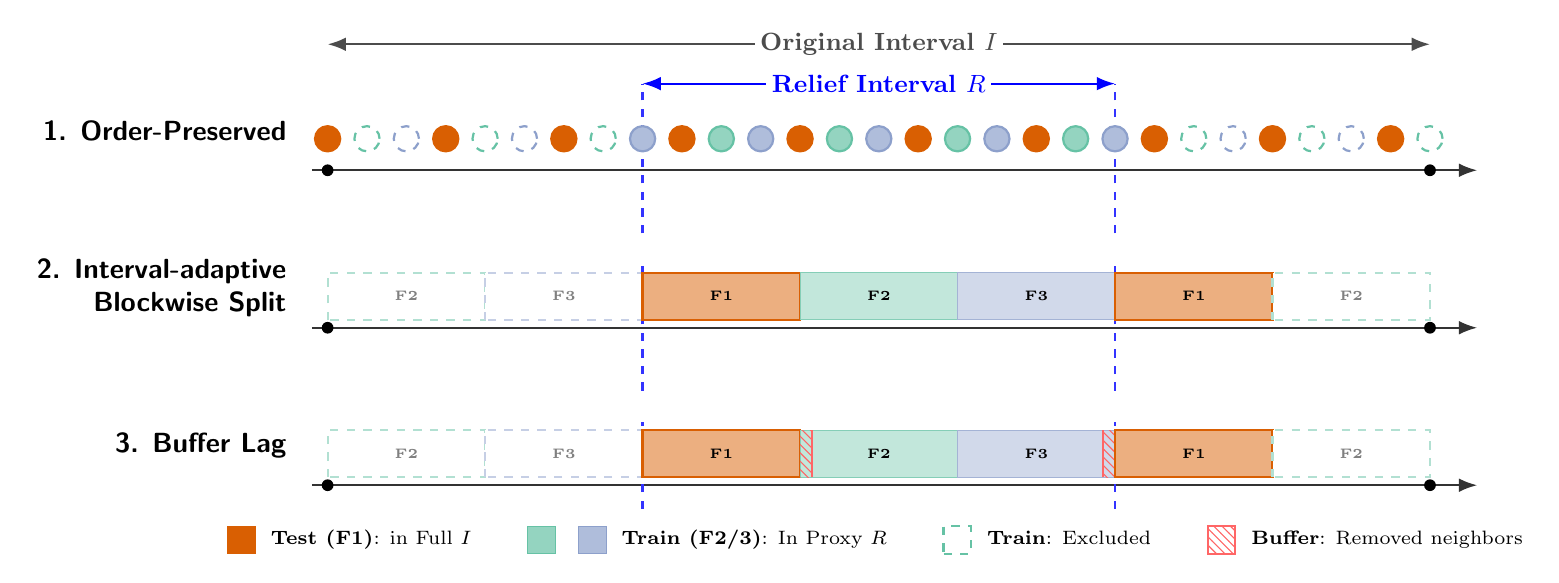
\begin{tikzpicture}[
    >=Latex,
    data_point/.style={
        circle,
        draw=black!50,
        thick,
        minimum size=0.32cm,
        inner sep=0pt,
        font=\tiny\bfseries
    },
    axis_style/.style={
        ->,
        thick,
        black!80
    },
    label_text/.style={
        font=\sffamily\bfseries,
        align=right,
        anchor=east
    },
    proxy_marker/.style={
        thick,
        blue!80,
        dashed
    },
    dim_line/.style={
        <->,
        thick
    }
]

    \definecolor{col1}{RGB}{102, 194, 165}
    \definecolor{col2}{RGB}{217, 95, 2}
    \definecolor{col3}{RGB}{141, 160, 203}


    \def\totalwidth{14}
    \def\proxystart{4}
    \def\proxyend{10}
    \def\sep{0.5}



    \def\yop{0}
    \node[label_text] at (-0.4, \yop + 0.5) {1. Order-Preserved};

    \draw[axis_style] (-0.2, \yop) -- (\totalwidth + 0.6, \yop);
    \node[circle, fill=black, inner sep=1.5pt] at (0, \yop) {};
    \node[circle, fill=black, inner sep=1.5pt] at (\totalwidth, \yop) {};


    \draw[dim_line, black!70] (0, \yop + 1.6) -- (\totalwidth, \yop + 1.6)
        node[midway, fill=white, inner sep=2pt, font=\small\bfseries] {Original Interval $I$};
    \draw[dim_line, blue] (\proxystart, \yop + 1.1) -- (\proxyend, \yop + 1.1)
        node[midway, fill=white, inner sep=2pt, font=\small\bfseries, text=blue] {Relief Interval $R$};
    \draw[proxy_marker] (\proxystart, \yop - 0.8) -- (\proxystart, \yop + 1.1);
    \draw[proxy_marker] (\proxyend, \yop - 0.8) -- (\proxyend, \yop + 1.1);


    \foreach \i in {0, ..., 28} {
        \pgfmathsetmacro{\xpos}{\i * \sep}
        \pgfmathparse{int(mod(\i, 3) + 1)} \let\foldid\pgfmathresult
        \pgfmathsetmacro{\inproxy}{\xpos >= \proxystart - 0.1 && \xpos <= \proxyend + 0.1 ? 1 : 0}
        \ifnum\foldid=1
            \node[data_point, fill=col2!100, draw=col2!100] at (\xpos, \yop + 0.4) {};
        \else
            \ifnum\inproxy=1
                \ifnum\foldid=2 \node[data_point, fill=col1!70, draw=col1!100] at (\xpos, \yop + 0.4) {}; \fi
                \ifnum\foldid=3 \node[data_point, fill=col3!70, draw=col3!100] at (\xpos, \yop + 0.4) {}; \fi
            \else
                \ifnum\foldid=2 \node[data_point, draw=col1!100, fill=white, dashed, thick] at (\xpos, \yop + 0.4) {}; \fi
                \ifnum\foldid=3 \node[data_point, draw=col3!100, fill=white, dashed, thick] at (\xpos, \yop + 0.4) {}; \fi
            \fi
        \fi
    }









    \def\yblk{-2}
    \node[label_text] at (-0.4, \yblk + 0.5) {2. Interval-adaptive\\Blockwise Split};

    \draw[axis_style] (-0.2, \yblk) -- (\totalwidth + 0.6, \yblk);
    \node[circle, fill=black, inner sep=1.5pt] at (0, \yblk) {};
    \node[circle, fill=black, inner sep=1.5pt] at (\totalwidth, \yblk) {};


    \draw[proxy_marker] (\proxystart, \yblk - 0.8) -- (\proxystart, \yblk + 0.8);
    \draw[proxy_marker] (\proxyend, \yblk - 0.8) -- (\proxyend, \yblk + 0.8);
    \pgfmathsetmacro{\blkwidth}{(\proxyend - \proxystart) / 3}
    \pgfmathparse{int(floor((0 - \proxystart) / \blkwidth))} \let\startidx\pgfmathresult
    \pgfmathparse{int(floor((\totalwidth - \proxystart) / \blkwidth))} \let\endidx\pgfmathresult

    \foreach \k in {\startidx, ..., \endidx} {
        \pgfmathsetmacro{\bstart}{\proxystart + \k * \blkwidth}
        \pgfmathsetmacro{\bend}{\proxystart + (\k + 1) * \blkwidth}
        \pgfmathparse{int(mod(mod(\k, 3) + 3, 3) + 1)} \let\foldid\pgfmathresult
        \pgfmathsetmacro{\drawstart}{max(0, \bstart)}
        \pgfmathsetmacro{\drawend}{min(\totalwidth, \bend)}

        \ifdim \drawstart pt < \drawend pt
            \pgfmathsetmacro{\bcenter}{(\drawstart + \drawend) / 2}
            \pgfmathsetmacro{\inproxy}{\bcenter >= \proxystart && \bcenter <= \proxyend ? 1 : 0}
            \ifnum\foldid=1
                \filldraw[fill=col2!50, draw=col2!100, thick] (\drawstart, \yblk + 0.1) rectangle (\drawend, \yblk + 0.7);
                \node[font=\tiny\bfseries] at (\bcenter, \yblk + 0.4) {F1};
            \else
                \ifnum\inproxy=1
                    \ifnum\foldid=2 \filldraw[fill=col1!40, draw=col1!80] (\drawstart, \yblk + 0.1) rectangle (\drawend, \yblk + 0.7); \fi
                    \ifnum\foldid=3 \filldraw[fill=col3!40, draw=col3!80] (\drawstart, \yblk + 0.1) rectangle (\drawend, \yblk + 0.7); \fi
                    \node[font=\tiny\bfseries] at (\bcenter, \yblk + 0.4) {F\foldid};
                \else
                    \ifnum\foldid=2 \filldraw[fill=white, draw=col1!50, dashed, thick] (\drawstart, \yblk + 0.1) rectangle (\drawend, \yblk + 0.7); \fi
                    \ifnum\foldid=3 \filldraw[fill=white, draw=col3!50, dashed, thick] (\drawstart, \yblk + 0.1) rectangle (\drawend, \yblk + 0.7); \fi
                    \node[font=\tiny\bfseries, text=gray] at (\bcenter, \yblk + 0.4) {F\foldid};
                \fi
            \fi
        \fi
    }


    \def\ybuf{-4}
    \node[label_text] at (-0.4, \ybuf + 0.5) {3. Buffer Lag};

    \draw[axis_style] (-0.2, \ybuf) -- (\totalwidth + 0.6, \ybuf);
    \node[circle, fill=black, inner sep=1.5pt] at (0, \ybuf) {};
    \node[circle, fill=black, inner sep=1.5pt] at (\totalwidth, \ybuf) {};


    \draw[proxy_marker] (\proxystart, \ybuf - 0.3) -- (\proxystart, \ybuf + 0.8);
    \draw[proxy_marker] (\proxyend, \ybuf - 0.3) -- (\proxyend, \ybuf + 0.8);
    \def\bufwidth{0.15}

    \foreach \k in {\startidx, ..., \endidx} {
        \pgfmathsetmacro{\bstart}{\proxystart + \k * \blkwidth}
        \pgfmathsetmacro{\bend}{\proxystart + (\k + 1) * \blkwidth}
        \pgfmathparse{int(mod(mod(\k, 3) + 3, 3) + 1)} \let\foldid\pgfmathresult
        \pgfmathsetmacro{\drawstart}{max(0, \bstart)}
        \pgfmathsetmacro{\drawend}{min(\totalwidth, \bend)}

        \ifdim \drawstart pt < \drawend pt
             \pgfmathsetmacro{\bcenter}{(\drawstart + \drawend) / 2}
             \pgfmathsetmacro{\inproxy}{\bcenter >= \proxystart && \bcenter <= \proxyend ? 1 : 0}
            \ifnum\foldid=1
                \filldraw[fill=col2!50, draw=col2!100, thick] (\drawstart, \ybuf + 0.1) rectangle (\drawend, \ybuf + 0.7);
                \node[font=\tiny\bfseries] at (\bcenter, \ybuf + 0.4) {F1};
            \else
                \ifnum\inproxy=1
                    \ifnum\foldid=2 \filldraw[fill=col1!40, draw=col1!80] (\drawstart, \ybuf + 0.1) rectangle (\drawend, \ybuf + 0.7); \fi
                    \ifnum\foldid=3 \filldraw[fill=col3!40, draw=col3!80] (\drawstart, \ybuf + 0.1) rectangle (\drawend, \ybuf + 0.7); \fi

                    \ifnum\foldid=3
                        \fill[pattern=north west lines, pattern color=red!60] (\bend - \bufwidth, \ybuf + 0.1) rectangle (\bend, \ybuf + 0.7);
                        \draw[red!60, thick] (\bend - \bufwidth, \ybuf + 0.1) -- (\bend - \bufwidth, \ybuf + 0.7);
                    \fi
                    \ifnum\foldid=2
                        \fill[pattern=north west lines, pattern color=red!60] (\bstart, \ybuf + 0.1) rectangle (\bstart + \bufwidth, \ybuf + 0.7);
                        \draw[red!60, thick] (\bstart + \bufwidth, \ybuf + 0.1) -- (\bstart + \bufwidth, \ybuf + 0.7);
                    \fi
                    \node[font=\tiny\bfseries] at (\bcenter, \ybuf + 0.4) {F\foldid};
                \else
                    \ifnum\foldid=2 \filldraw[fill=white, draw=col1!50, dashed, thick] (\drawstart, \ybuf + 0.1) rectangle (\drawend, \ybuf + 0.7); \fi
                    \ifnum\foldid=3 \filldraw[fill=white, draw=col3!50, dashed, thick] (\drawstart, \ybuf + 0.1) rectangle (\drawend, \ybuf + 0.7); \fi
                    \node[font=\tiny\bfseries, text=gray] at (\bcenter, \ybuf + 0.4) {F\foldid};
                \fi
            \fi
        \fi
    }



    \node[anchor=north, align=center, font=\scriptsize, inner sep=0pt] at (\totalwidth/2, \ybuf - 0.5) {
        \legendBox{fill=col2!100, draw=col2!100} \textbf{Test (F1)}: in Full $I$
        \hspace{1.5em}
        \legendBox{fill=col1!70, draw=col1!100} \legendBox{fill=col3!70, draw=col3!100} \textbf{Train (F2/3)}: In Proxy $R$ \hspace{1.5em}
        \legendBox{draw=col1!100, fill=white, dashed, thick} \textbf{Train}: Excluded
        \hspace{1.5em}
        \legendBox{draw=red!60, thick, pattern=north west lines, pattern color=red!60} \textbf{Buffer}: Removed neighbors
    };

\end{tikzpicture}

\end{document}